%%%%%%%%%%%%%%%%%%%%%%%%%%%%%%%%%%%%%%%%%%%%%%%%%%%%%%%%%%%%%%%%%
% !TEX root = interimreport.tex
\clearpage
\chapter{NEW INSTRUCTIONS}\label{Ch9}
%%%%%%%%%%%%%%%%%%%%%%%%%%%%%%%%%%%%%%%%%%%%%%%%%%%%%%%%%%%%%%%%%

\section{SHLXOR Instruction}
We extended the instruction set by adding the SHLXOR instruction. The purpose of this instruction is to shift the first source operand one bit to the left and then XOR it with the second source operand. Then, the obtained result is stored in the destination register. By adding this instruction, we can perform this operation with a single instruction instead of using shift left and XOR instructions separately, making it more efficient.
Let’s give an example to make it clearer what this instruction does. RS1 and RS2 are source operands and RD is the output.
RS1: 0x0101     RS2: 0xFFFF     RD: 0xFDFD
0x0101 is shifted left by one and then XOR’ed with 0xFFFF, giving the result 0xFDFD.
As we mentioned, this new instruction requires two source registers and one destination register. Therefore, unlike the MLA instruction, we don’t need to create a new class to support it. There is already a class named ALU\_rr in the RISCVInstrinfo.td file which has two source and one destination register. Therefore, the new SHLXOR instruction is going to belong to the ALU\_rr class. The ALU\_rr class is given below.

\begin{lstlisting}
let hasSideEffects = 0, mayLoad = 0, mayStore = 0 in
class ALU_rr<bits<7> funct7, bits<3> funct3, string opcodestr,
bit Commutable = 0>
: RVInstR<funct7, funct3, OPC_OP, (outs GPR:\$rd), (ins GPR:\$rs1, GPR:\$rs2),
opcodestr, "\$rd, \$rs1, \$rs2"> {
let isCommutable = Commutable;
}
\end{lstlisting}

As we can see, encoding of this type of instructions consists of funct7, funct3, opcode, source registers, and the destination register. The encoding format and the other properties are described in the class. The source registers are described as inputs and the destination register is described as the output.
In the RISCVInstrInfoCrypt.td file, we add the definition of the SHLXOR instruction by using the ALU\_rr class. In this part, we define funct7, funct3, and the mnemonic of the new instruction as well as the schedulings.

\begin{lstlisting}
def SHLXOR : ALU_rr<0b0011000, 0b111, "shlxor">,
Sched<[WriteIALU, ReadIALU, ReadIALU]>;
\end{lstlisting}

Also in the same file, we define the instruction’s pattern. When we examine this definition, we can clearly see what the instruction performs and its pattern. In the inner parentheses, we can see the shifting of the first source operand by one bit. Then, the result of this shifting operation is used as an input for the XOR operation alongside the second source operand.

\begin{lstlisting}
def : Pat< (xor (shl GPR:\$src1, (i32 1)), GPR:\$src2),
(SHLXOR GPR:\$src1, GPR:\$src2)>;
\end{lstlisting}

After doing these, we can try it with a simple C code given in \ref{fig:c_code_for_shlxor}. Let’s get an assembly output from the C code by running the following commands:

\begin{lstlisting}
clang -S -target riscv32-linux-gnu -emit-llvm -g shlxor.c
$~/CustomInstrLLVM/build/bin/llc -mtriple=riscv32 shlxor.ll$
\end{lstlisting}

Here, CustomInstrLLVM is the folder that we built llvm in.

\begin{figure}
    \centering
    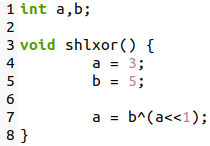
\includegraphics{adding_new_instr/c_code_for_shlxor.png}
    \caption{C code for SHLXOR}
    \label{fig:c_code_for_shlxor}
\end{figure}

This C code basically shifts the variable a by one bit and XOR’s it with b variable. Then the result is stored in a. We can see that, the register that stores the value a is both the first source register and the destination register. The assembly output is given in figure \ref{fig:shlxor_assembly_output}.
\begin{figure}
    \centering
    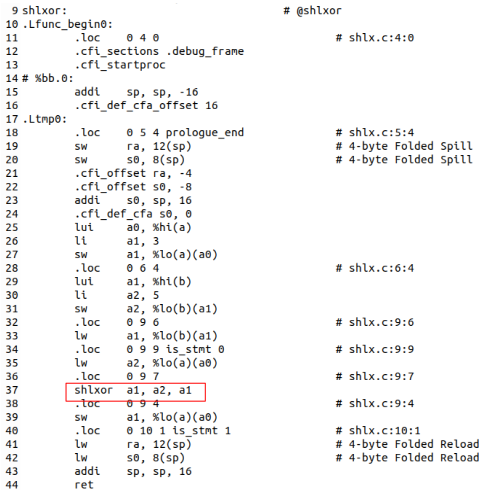
\includegraphics{adding_new_instr/shlxor_assembly_output.png}
    \caption{SHLXOR assembly output}
    \label{fig:shlxor_assembly_output}
\end{figure}

In the assembly output, we can see the SHLXOR instruction. a1 and a2 are the sources and a1 is also the destination as we can see.

\section{RORI Instruction}
One of the Instructions that we worked on is RORI instruction. The purpose of this instruction is to take the operand and rotate it to the right by the amount of the immediate value. This is different from shifting right using an immediate. When shifting a number to the right, the rightmost (least significant) bits are deleted and the leftmost (most significant) bits are filled in with zeros. On the other hand, when a number is rotated right, the least significant bits that are pushed out are not deleted but written into the most significant bits. We want to add add an instruction that performs this operation.

First of all, we tried pattern matching and added the definition and pattern of our new instruction to the InstrInfoCrypt.td file. However, that didn’t work and we couldn’t see the RORI instruction when we checked our assembly output created by using a simple C code that implements the rotation operation. This is because the pattern can have different combinations and may not match with what we expect. Therefore, the instruction cannot be recognized and we can’t see it in the assembly output.

Realizing that, we looked for other options and tried to make use of intrinsics and builtin functions. We added the definitions into the InstrInfoCrypt.td file.

\begin{lstlisting}
def ROTI : ALU_ri<0b101, "roti">;
\end{lstlisting}

It is ALU\_ri type because one of the operands is an immediate value and we only need one register for this instruction.

\begin{lstlisting}
def : Pat<(rotr GPR:\$rs1, simm12:\$imm12),
(ROTI GPR:\$rs1, simm12:\$imm12)>;
\end{lstlisting}

We used rotr here because we wanted to make use of the builtin function \_\_builtin\_rotateright32. rotr is defined in the RISVIselLowering.cpp file.

\begin{lstlisting}
if (Subtarget.hasStdExtZbb() || Subtarget.hasStdExtZbkb()) {
if (Subtarget.is64Bit())
setOperationAction({ISD::ROTL, ISD::ROTR}, MVT::i32, Custom);
} else {
setOperationAction({ISD::ROTL, ISD::ROTR}, XLenVT, Expand); 
}
\end{lstlisting}

However, we need to change the “Expand” to “Legal” in here otherwise we will not see the ROTI instruction in the assembly output.  This way, we are legalizing the action. If we don’t do this, we will see the fshr (funnel shift right) intrinsic in the .ll file but ROTI won’t make it into the assembly output. After doing these, we can try it with a simple C code. As mentioned before, we used a built in rotate function in the C code given in figure \ref{fig:c_code_with_builtin_function_for_roti}.
\begin{figure}
    \centering
    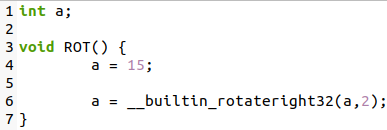
\includegraphics{adding_new_instr/c_code_with_builtin_function_for_roti.png}
    \caption{C code with builtin function for RORI}
    \label{fig:c_code_with_builtin_function_for_roti}
\end{figure}

This code rotates 15 to the right by 2 bits. We can obtain the .ll file given in figure \ref{fig:rotill_output_for_rotic} by running the following command.

\begin{lstlisting}
clang -S -target riscv32-linux-gnu -emit-llvm -g roti.c
\end{lstlisting}

\begin{figure}
    \centering
    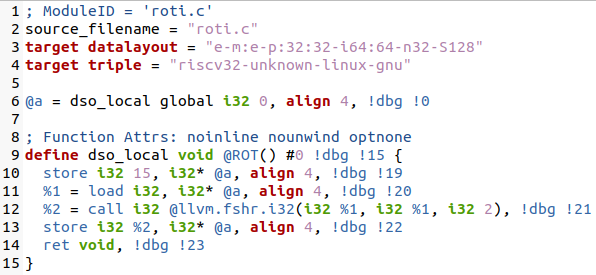
\includegraphics{adding_new_instr/rotill_output_for_rotic.png}
    \caption{roti.ll output for roti.c}
    \label{fig:rotill_output_for_rotic}
\end{figure}

The fshr intrinsic is visible in the twelfth line. After that, the assembly output can be obtained by running the following command. The assembly output is given in figure \ref{fig:roti_assembly_output}.

\begin{lstlisting}
$~/CustomInstrLLVM/build/bin/llc -mtriple=riscv32 roti.ll$
\end{lstlisting}

\begin{figure}
    \centering
    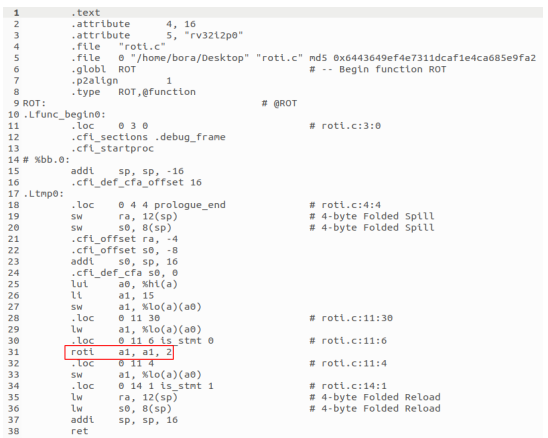
\includegraphics{adding_new_instr/roti_assembly_output.png}
    \caption{ROTI assembly output}
    \label{fig:roti_assembly_output}
\end{figure}

The ROTI instruction can be seen in the assembly output. As expected, it uses one register as both  the destination and the source alongside an immediate value.

This way, we succesfully obtained the ROTI instruction. However, using the builtin function while writing the C code wasn’t the prettiest solution. Therefore, we looked further into how we can implement this. After that, we realized that there is a bit manipulation extension for RISCV and what we need was in the RISCVInstrInfoZb.td file. This file contains the instruction extensions for bit manipulations. These instructions operate on the bits of the data and RORI is one of those instructions. However, in order to utilize this extension, we need to add some flags to the command while running clang in order to get an assembly output from the C code we write. The simple C code for RORI is given in figure \ref{fig:c_code_for_rori}.
\begin{figure}
    \centering
    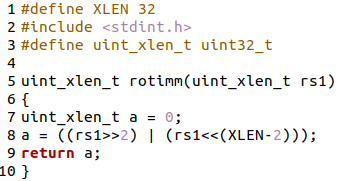
\includegraphics{adding_new_instr/c_code_for_rori.png}
    \caption{C code for RORI}
    \label{fig:c_code_for_rori}
\end{figure}

Here, we use 32 as the length because our target is 32 bit and the rotation is implemented in the eighth line. After that, we run the following command with additional flags as mentioned before.

\begin{lstlisting}
$clang --target=riscv32 -O -S rori.c -march=rv32imaczbb$
\end{lstlisting}

Here, -O defines the level of optimization. -S is used for getting an assembly file as an output. rori.c is the name of our simple C code. -march=rv32imaczbb designates that we want to utilize the zbb subgroup of the bit manipulation extension. The assembly output is given in figure \ref{fig:rori_assembly_output}.
\begin{figure}
    \centering
    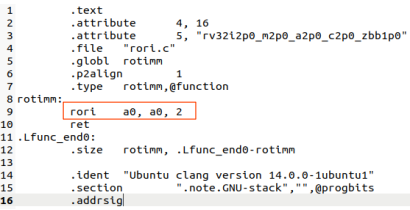
\includegraphics{adding_new_instr/rori_assembly_output.png}
    \caption{RORI assembly output}
    \label{fig:rori_assembly_output}
\end{figure}

This way, we managed to succesfully obtain RORI instruction in the assembly output.
